% !TeX spellcheck = en_US
\documentclass[11pt,a4paper,oneside,openright,titlepage]{article}

\usepackage[utf8]{inputenc}
\usepackage[english]{babel}
\usepackage{amsmath}
\usepackage{mathtools}
\usepackage{amsfonts}
\usepackage{amssymb}
\usepackage{listings}  % Required for insertion of code
\usepackage{graphicx} % Required to insert images
\usepackage{textcomp}
\usepackage{enumerate} % Required for enumerate model
\usepackage{gensymb} %Required for degree symbol which is made ^{\circ}
\usepackage{caption} %used to have cool captions
\captionsetup{
	tableposition=top,
	figureposition=bottom,
	font=small,
	format=hang, 
	labelfont=bf}	%caption setup
\usepackage[protrusion=allmath]{microtype} %used to have high quality text formatting
\usepackage{graphicx,subfig,float,wrapfig,rotating,multirow,epstopdf} %high quality tables and images formatting
\usepackage{booktabs,siunitx,array,tabularx} % tables
\usepackage{amsbsy,bm,amsmath} % math

%\usepackage [ Lenny ]{fncychap}
\usepackage{longtable} % Required to put long tables
\usepackage{float} 
\usepackage{hyperref} % next packages are used to have navigation tree in pdf reader
\hypersetup{pdftex,colorlinks=true,allcolors=black}
\usepackage{hypcap}

\usepackage{amsmath}
\usepackage{cancel}
\usepackage{gensymb}
\usepackage[utf8]{inputenc}
\usepackage{xstring}
\usepackage[]{circuitikz}

\newcommand{\facciatabianca}{\newpage\shipout\null}


\lstset{ % Frame for Matlab code
	numbers=left, 
	numberstyle=\small, 
	numbersep=8pt, 
	frame = single, 
	language=Matlab, 
	framexleftmargin=19pt,
	breaklines}

\pagestyle{plain}

\graphicspath{{img/}} % Set graphics directory

\def\permille{\ensuremath{{}^\text{o}\mkern-5mu/\mkern-3mu_\text{oo}}} % Add symbol of per mille
\newcommand{\parallelsum}{\mathbin{\!/\mkern-5mu/\!}} % Fix parallel symbol inclination

%\makeindex

\title{	Analog Integrated Circuits \\
	\huge {\textsc{Analysis and design of a double balanced Gilbert Cell Based Mixer in AMI06 technology}}	}
 	
\begin{document}
\author{Enrico Maria Renzi \\Roberto Rubino\\}
\date{\today}


\maketitle	
\newpage
\thispagestyle{empty}
\clearpage\mbox{}\clearpage



\tableofcontents
\pagenumbering{roman}

\newpage
\thispagestyle{empty}
\clearpage\mbox{}\clearpage

\pagenumbering{gobble}
\section*{}
\begin{flushright}
\textbf{DA SISTEMARE}
	There are many deadlocks and
	dependencies which have to be taken into consideration while designing the specifications
	for the transistors in order to satisfy the above design constraints. All the calculated
	values are changed based on the parametric analysis of transistors in Cadence Virtuoso.
\end{flushright}\newpage
\newpage
\thispagestyle{empty}
\clearpage\mbox{}\clearpage
\pagenumbering{arabic}
% nel mixer bisogna aggiungere x(t), y(t) in ingresso e z(t) in uscita e aggiungere freccia


\section{Introduction}
\begin{figure}[H]
	\centering
	\scalebox{1.3}
{
	\begin{circuitikz} 
		\ctikzset{tripoles/mos style/arrows,bipoles/length=1cm}
		\draw
		(0,0) node[mixer] (m) {}
		(m.1) to[short,-] ++(-.5,0) node[left]{$x_1(t)$}
		(m.2) to[short,-] ++(0,-.5) node[below]{$x_2(t)$}
		(m.3) to[short,-] ++(.5,0) node[inputarrow]{} (.5,0) node[right=3mm]{$y(t)$}
		(m.1) node[inputarrow] {} 
		(m.2) node[inputarrow,rotate=90] {};
	\end{circuitikz}
}		
\caption{Representation of a mixer}
\label{Mixer}
\end{figure}
An analog multiplier, also known as mixer, is a circuit that performs the product between two signals. As we will see, this feature can be exploited to convert informations from a certain frequency band to another by means of the intrinsic non-linear behaviour of this net. Supposing to have two sinusoidal signals
\begin{align}
x_1(t) &= A_1 \cos(\omega_1 t + \varphi_1) \notag \\
x_2(t) &= A_2 \cos(\omega_2 t + \varphi_2) \notag
\end{align}
and the ideal mixer shown in figure \ref{Mixer} has that the out-coming signal $y(t)$ is given by:
\begin{align}
y(t)& =x_1(t)\cdot x_2(t)   \notag \\
& = A_1 A_2 \cos(\omega_1 t + \varphi_1) \cos(\omega_2 t + \varphi_2) \notag \\
& = \frac{A_1 A_2}{2} \{\cos[(\omega_1-\omega_2) t + \varphi_1-\varphi_2]+ \cos[(\omega_1+\omega_2) t +\varphi_1+ \varphi_2]\} \notag \\
& = A \cos(\omega_{LF} t + \varphi_{LF}) + A \cos(\omega_{HF} t + \varphi_{HF}) \notag
\end{align}
where
\begin{align}
\omega_{LF}&= |\omega_1-\omega_2| \notag \\
\omega_{HF}&= |\omega_1+\omega_2| \notag \\
\varphi_{LF} &= \varphi_1-\varphi_2 \notag \\
\varphi_{HF} &= \varphi_1+\varphi_2 \notag 
\end{align}
Therefore, it comes that two signals with different frequency allocation are obtained at the output port: the former at $\omega_{LF}<\omega_1,\omega_2$ will be the down-converted component whereas the latter, with $\omega_{HF}>\omega_1,\omega_2$, will be the up-converted one.  Moreover, it is possible to select only one of these two signals by properly filtering out the unwanted part.
Overall one can read the process as a modulation of an input signal by means of a carrier.  Since the mixer is a bidirectional three-port, one can distinguish: 
\begin{itemize}
	\item The high frequency signal, RF. In case of down-conversion this is one input of the circuit, vice-versa it is the output (after filtering).
	\item The intermediate frequency signal, IF. In case of up-conversion this is one input of the circuit, vice-versa it is the output (after filtering).
	\item The local oscillator, LO. This is the carrier and it is always an input with known frequency.
\end{itemize}

Based on the above, it turns out that to mix-up two signals a non-linear device is needed, since the input components are at different frequency with respect to the output and a non-linear relation between voltages and currents appears. In general, mixing can be carried out by time-varying systems that can be implemented using:
\begin{description}
	\item [passive devices]	typically switches (diodes and transistors). In this case the mixing process introduces a \emph{loss} since the output power is always less than the input one.
	\item [active devices] amplifying devices are used in active region providing \emph{gain}.\footnote{The definition of the gain and loss in mixer is different with respect to the one of linear devices, and will be discussed further.} They are more power consuming and less noisy than passive mixers.
\end{description}
Another way to classify mixers is the following:
\begin{description}
	\item [Single balanced mixers] One or both input signals can pass to output, but it is not possible to suppress both of them,
	\item [Double balanced mixers] Thanks to symmetry in the net both the input and the LO are rejected at the output port. They show better isolation between ports than SBM. 
\end{description}
To understand why a transistor can be used, let's consider the non-linear quadratic model for a nMOSFET. Supposing to drive it by injecting a two tone signal $v_{GS}(t)=v_{RF}(t)+v_{LO}(t)$ at the gate (down-conversion configuration). One has:
\begin{align}
i_D(t) &= k(v_{GS}(t)-V_{th})^2 \notag \\
& = k(v_{RF}(t)+v_{LO}(t)-V_{th})^2 \notag \\
& = k[v_{RF}^2(t)+v_{LO}^2(t)+2v_{RF}(t)v_{LO}(t)-2(v_{RF}(t)+v_{LO}(t))V_{th}+V_{th}^2)] \notag
\end{align}
Supposing now $v_{RF}<<v_{LO}$:
\begin{align}
i_D(t) &\simeq k(v_{LO}(t)-V_{th})^2+2k(v_{LO}(t)-V_{th})v_{RF}(t) \notag  \\
& = I_D(t)+g_m(t)v_{RF}(t) \notag
\end{align}
hence, the model becomes a \emph{quasi-linear} time-varying \emph{small signal model} and the device operates in the \emph{Small Signal Large Signal} regime (SSLS), because we still have the product of the two input signals through the transconductance. It is worth it to notice that depending on the amplitude of the RF (the LO is always driven in large signal), mixing can be obtained both in linear region or through second order non-linearity (fully non-linear device).
A more detailed analysis about how to drive a mixer follows in section 2.

Similarly to linear circuits, even in case of mixers it is possible to define the gain. Actually, gain is defined only in case of linear systems, but this figure of merit is necessary to qualify the performance of the conversion stage.
In case of non-monochromatic signals (general case) one defines the \emph{voltage conversion gain} as:
\begin{equation}
	A_v= \frac{V_{IF,rms}}{V_{RF,rms}} \notag
\end{equation}
moreover, one has that the output power is proportional to LO power (that is also called a \emph{pump}), even if this dependency does not appear explicitly.

An important figure of merit concerning mixers is given by the 1dB compression point of the $P_{in}$/$P_{out}$ characteristic. By increasing the value of the RF signal, the amount of harmonics at the output besides the fundamental IF frequency increases as well, eventually saturating the output (gain compression or flatness). This is due to the fact that power is no more mainly carried by the fundamental output tone (i.e. the IF tone), but it is rather shared by all the growing up harmonics. In other words the conversion gain stops to be constant, reduces itself, and the output waveform is clipped. Supposing to have input and output impedance matching one has that:
\begin{align}
	A_{conv}&=\frac{P_{IF}}{P_{RF}} \notag \\
	10\log_{10}A_{conv} & = 10\log_{10}\frac{P_{IF}}{P_{RF}}  \notag \\
	10\log_{10}P_{IF} & = 10\log_{10}A_{conv} + 10\log_{10}P_{RF} \notag \\	P_{IF}|_{dB_{m}} &= A_{conv}|_{dB} + P_{RF}|_{dB_{m}}+30dB \notag
\end{align}
This suggests both that the ideal output characteristic looks linear in log scale until the gain does not compress and that the 1dB compression point can be defined as the output IF voltage at which:
\begin{equation}
P_{IF}|_{-1dB} = A_{conv}|_{dB} + P_{RF}|_{dBm} -1dB \notag
\end{equation}
hence:
\begin{equation}
P_{IF}|_{-1dB} = P_{IF}|_{dB_{m},ideal} -1dB \notag
\end{equation}

Other important figures of merit concern the third order distortions, that can be defined as follow:
\begin{description}
	\item [Third Order Distortion] In this case the input is a monochromatic signal. Because of the intrinsic device's non-linearity, the output signal contains frequency components not present at the input. It can be demonstrated that the most important spurious contribution on output fundamental tone comes from the third order term, in fact, by expanding the device's output current in Taylor's series and supposing a monochromatic gate signal, one has:
	\begin{align}
		i_D(t) &= I_D|_{V_{GS}}+av_{gs}(t)+bv_{gs}^2(t)+cv_{gs}^3(t)+\dots \notag \\
		&=I_D|_{V_{GS}}+i_{D,fund}(t)+i_{D,SOD}(t)+	i_{D,TOD}(t)+\dots
	\end{align}
	Where $a>b>c$. Developing the first three terms of the series expansion one has:
	\begin{align}
	&i_{D,fund}(t) \propto a\cos(\omega_0 t) \\
	&i_{D,SOD}(t) \propto b\cos^2(\omega_0 t) =\frac{1}{2}b+\frac{1}{2}b\cos(2\omega_0 t) \\
	&i_{D,TOD}(t) \propto c\cos^3(\omega_0 t) = \frac{3}{4}c\cos(\omega_0 t) +\frac{1}{4}c\cos(3\omega_0 t)
	\end{align} 
	It is straightforward that the third order term yields an additive contribution exactly at the fundamental tone, whereas the second order distortion adds a zero-frequency term that is not interfering with in-band signal (a balanced configuration can reject DC component). In general, even order distortions (2\textsuperscript{nd}, 4\textsuperscript{th} \dots) contributes in corrupting the output signal as well, though they are less important. Also 5\textsuperscript{th} order distortion exist, for which the same reasoning holds. Since the whole signal is mixed, all the additional tones introduced by distortion are moved in frequency and they may produce in-band spurious components.
	
	\item [Third Order Intermodulation, IM\textsubscript{3}] This distortion comes from a two-tone input injection ($f_1 = f_0$ and $f_2=f_0+\delta f$). Due to intermodulation between tones, unwanted frequencies are generated. The most important contribution comes from the third order intermodulation (IM3): $|m|+|n|=3$ and $m\cdot n<0$ (where $m=\pm2,\pm1$ and $n=\pm2,\pm1$ are the intermodulation indexes). Taking $m=2$ and $n=-1$:
	\begin{equation}
		f_{IM3}|_{m=2,n=1} =  2f_1 - f_2 = f_0 - \delta f \notag
	\end{equation}
	that is clearly an in-band distortion.
	It can be demonstrated (FONTE) that, in case of same input and output reference impedance, the out and in intermodulation points are related to stage gain and output power of first harmonic:
	\begin{gather}
	OIP_3|_{dB} = \frac{3}{2}P_{out,1st}|_{dB}-\frac{1}{2}P_{out,IM3}|_{dB} \notag \\
	IIP_3|_{dB} = OIP_3|_{dB}-A_{v,1st}|_{dB} \notag
	\end{gather} 
	By taking $m=-1$ and $n=2$ one has instead:
	\begin{equation}
	f_{IM3}|_{m=-1,n=2} =  -f_1 +2 f_2 = f_0 + \delta f \notag
	\end{equation} 
	We notice that the whole spectrum presents side-bands produced by intermodulation. This phenomenon is called \emph{spectral regrowth} and it can be quantified by the \emph{Carrier to Intermodulation Ratio (CIM)}.
	In case of mixing we change frequency band from input to output, anyway the previous result holds:
	\begin{gather}
			f_{IF,IM3}|_{m=2,n=-1} = 2f_{RF1} - f_{RF2} -f_{LO}= f_{IF} - \delta f \notag
	\end{gather}
\end{description}

\textbf{DA FINIRE CON FIGURE DI MERITO}\newpage
\section{Analysis of a Gilbert cell-based multiplier }

\subsection{Gilbert cell overview}
A CMOS-based technology Gilbert cell-based mixer is shown in figure \textbf{AGGIUNGI IMMAGINE}. This circuit exploits a differential topology to implement a double-balanced cell providing:
\begin{itemize}
	\item Reasonable conversion gain (from one to some tens);
	\item Thanks to the double-balanced topology if performs good rejection of input frequency components to the output port along with high linearity;\footnote{The linearity is meant with respect to the conversion gain.}
	\item Good isolation between ports is provided by the high suppression of spurious frequency components;
	\item Thanks to the CMOS architecture it can be integrated.
\end{itemize}
\subsection{Gilbert cell circuit analysis}
To analyse the circuit it is necessary to give some informations about its topology, polarization and driving. Looking a FIGURA DOVE C'E' MIXER COMPLETO it is possible to identify five main blocks that are described in what follows.
\paragraph{Bias net}

This net is made up of the current mirror (transistors M1 and M2) and the voltage reference generation branch (transistor M5, R1, R2, R3, R4, R5). 

Transistor M1 is the strong branch of the current mirror and it acts as a current sink for the differential pair made up by M3 and M4, fixing the polarization current for the whole circuit. M2 sinks instead the current from the voltage reference section of the bias net.
Generally transistors in current mirrors are polarized in saturation region, so that an high output resistance is seen from the stage above: this means that M1 should appear as a good current sink.
Given $V_{G1}=V_{GS1}$ the gate voltage in M1 we have that the transistor remains in saturation if:
\begin{gather}
\label{eq:sat_m1}
V_{GS}\geq V_{th}  \\
V_{DS}>V_{od} = V_{GS}-V_{th} 
\end{gather}
The same holds for M2, that is always in saturation condition since it is diode connected (provided \ref{eq:sat_m1}). In saturation (neglecting channel modulation effects), one has that the drain current only depends on gate voltage and it is given by:
\begin{equation}
\label{eq:Id_quadLaw}
I_D = \mu_{n,eff} \frac{C_{ox}}{2} \frac{W}{L} (V_{GS}-V_{th})^2 = \frac{\beta_{n}}{2}V_{od}^2
\end{equation}
hence M1 remains in saturation till when:
\begin{equation}
V_{DS1}\geq V_{od1}= V_{th}-\sqrt{\frac{2I_0}{\beta_{n}}}
\end{equation}
therefore to have a low value of the overdrive voltage one should have large transistors, i.e. large W.
The output resistance in instead defined by:
\begin{equation}
 r_o = \frac{1}{\lambda I_0} \propto L
\end{equation}
where $\lambda$ takes count of the channel modulation. It appears that we need long transistors to have better current sink's properties.
By looking at FIGURE 2, one has (supposing both M2 and M1 in saturation, and $V_{GS1}=V_{GS2}=V_{DS1}=V_{DS2}$):
\begin{gather}
I_0 = \frac{\beta_{n1}}{2}(V_{GS1}-V_{th})^2(1+\lambda_1V_{DS1}) \notag \\
I_{REF} = \frac{\beta_{n2}}{2}(V_{GS1}-V_{th})^2(1+\lambda_1V_{GS1}) \notag
\end{gather}
hence, supposing to have equal transistors:
\begin{equation}
\frac{I_0}{I_{REF}} = \frac{W_1/L_1}{W_2/L_2} 
\end{equation}
Ideally the current mirroring is only depending on geometrical parameters, this means that a very good matching is required. Even if the two devices are very close to each other within the same chip, it exists the possibility to have a variation in parameters that depend on temperature, i.e. $V_{th}$ and $\mu_{n,eff}$. Supposing to have equal devices with everything constant but:
\begin{gather}
K_{n1}=K_n+\Delta K_n \notag \\
V_{th,1} = V_{th}+\Delta V_{th} \notag
\end{gather}
one eventually finds that:
\begin{equation}
\frac{I_0}{I_{REF}} \simeq 1 + \frac{\Delta K_n}{K_n}+2\frac{\Delta V_{th}}{V_{od}} \notag
\end{equation}
Then, some of the possible mismatch causes are:
\begin{itemize}
	\item $K_n$, that can varies a lot in case of wide circuits;
	\item $V_{od}$ that usually is set low and varies with $V_{th}$, whose small variation can produce large differences in the two currents;
	\item difference between $V_{DS1}$ and $V_{DS2}$.
\end{itemize}
Assuming as maximum variations:
\begin{gather}
\frac{\Delta K_n}{K_n} = \pm 5 \% \notag \\
\frac{\Delta V_{th}}{V_{GS}-V_{th}} = \pm 10 \% \notag
\end{gather}
one has:
\begin{equation}
\frac{I_0}{I_{REF}} = 1 \pm 15 \% \notag
\end{equation}
A cascaded voltage divider is connected as M2's load: 
\begin{itemize}
	\item M5 is diode connected and it is used to generate the right gate bias voltage for the gain stage.
	\item A resistive voltage divider made up of R2 and R4 is used to polarize the mixing stage.
	\item Resistors R1 and R3 are used to connect the bias net to the gain and mixing stages' gates. They also acts as high impedance for the RF and LO signals coming from outside the circuit and prevents them to enter the bias net.
	\item Capacitors C1 and C2 shunt possible non-DC disturbances coming from the Gilbert Cell, improving the bias isolation.
\end{itemize}

Noise issues will not be analysed within this treatise, it should be considered for a more complete design though. As a rule of thumb, narrow gate and low overdrive voltages should used to lower noise contribution.(FONTE) 
Using a resistive voltage reference can be detrimental in case of voltage supply fluctuation, since a resistive voltage divider cannot reject current variations. However using active devices we would produce much more noise injection within the net though.

\paragraph{Gain stage}

The gain stage (shown in figure 3) is the linear part of the mixer, it must handle without distortion and corruptions the power coming from the RF signal giving some amplification. The topology is suited for a low noise amplifying purpose (FONTE): a differential stage with source degeneration. The stage is made up of two transistors (M3 and M4) in common source configuration directly polarized by M1 and two source degeneration resistances $R_S$.

The RF differential signal modulates the current flowing into each of the two transistors, that has to be polarized in saturation region. For both of them it must be ensured an high output voltage range and a quite low overdrive voltage, along with a large drain to source bias voltage (required to maintain the stage in saturation during the swing of the LO stage).

To have an idea on the gain that can be obtained by this stage, one can look at the stage in FIGURE 3. Removing the degeneration resistances one has that the gate-to-gate mesh gives:
\begin{equation}
V_{in,1}-V_{in,2} = V_{GS3}-V_{GS4} \notag
\end{equation} 
from equation \ref{eq:Id_quadLaw}, recalling that $I_{1}+I_{2}=I_0$ and squaring:
\begin{equation}
(V_{in,1}-V_{in,2})^2 = \frac{2}{\beta_n}(I_0-2\sqrt{I_1 I_2}) \notag
\end{equation}
that once inverted yields
\begin{equation}
I_{1}-I_{2} = \sqrt{\beta_n I_0}(V_{in,1}-V_{in,2})\sqrt{1-\frac{\beta_n}{4I_0}(V_{in,1}-V_{in,2})^2} \notag
\end{equation}
writing the previous equation in term of $\Delta I =I_{1}-I_{2} $ and $\Delta V_{in} = V_{in,1}-V_{in,2}$ and computing the value of the slope ot this characteristic, one obtains that the maximum differential voltage gain in equilibrium condition $\Delta V_{in} =0$ is given by:
\begin{equation}
\label{eq_statiGain}
|A_{v}|= \sqrt{\beta_{n}I_0}R_1
\end{equation}
This suggest that it is better to polarize the stage exactly with  $V_{GS1}=V_{GS2}$. The complete expression for equation \ref{eq_statiGain} also gives that the differential transconductance is a strongly non-linear function of the gate bias voltage. 

As we said before there it is the possibility to have a mismatch between the transistors and the loads due to circuit dimensions, temperature distribution and process tolerances, then looking at FIGURE 3:$M3 \neq M4$ and $R1 \neq R2$. It can be demonstrated that the offset output voltage due to differences in the circuit parameters and dimensions is:
\begin{equation}
V_{o,offset}= \Delta V{th}+\frac{V_{GS}-V_{th}}{2}\Bigg(-\frac{\delta R}{2R}\frac{\Delta W /L}{2W/L}\Bigg) \notag
\end{equation}
To reduce this error a common centroid topology should be used in layout.
Besides, it is important to notice that R1 and R2 are both the source output conductance of a common gate stage (mixing stage of the Gilbert cell) and that the actual gain for the RF stage is a current gain. 

The small signal equivalent transconductance of the stage, once we added the source degeneration, (APPENDICE?) is given by:
\begin{equation}
\label{eq_degenGain}
G_{eq} = \frac{g_m}{1+g_m R_S}
\end{equation}
By adding $R_S$ we lower the RF stage's current gain, however  we also get a more linear behaviour reducing its dependency with respect to bias point (this fact will be demonstrated later). LINEARITA' CON OVERDRIVE?? (RAZAVI rf PAG 193)

\paragraph{Mixing stage}
This stage is also called \emph{switching stage}, suggesting the way we want to drive transistors M6 to M9 (FIGURE 4). Also this one has a differential topology, however, differently from the RF stage, we drive each pair with complementary LO signals that turn on and off cycle-by-cycle one of the two devices. The driving signal il sinusoidal (similarly one can apply a square wave) and it must be large enough to ensure the abrupt switching of the stage: when a device is on it must be in saturation (not in  triode!), while the other one must be completely of, interdicted.
A compromise is needed since:
\begin{itemize}
	\item small amplitude of LO signals produce slower switching speed, hence part of the power is wasted as common mode signal at the output;
	\item too large LO signals drive the MOSFET in triode region producing spikes that corrupt the output signal with unwanted feed-through  and reduces speed.
\end{itemize}
Switching speed is related to the device cut-off frequency, that for short channel devices is inversely proportional to channel length and linearly dependent to the overdrive voltage:
\begin{equation}
f_T \propto  V_{od}/L \notag
\end{equation}
suggesting that the highest overdrive and the minimum channel length should be chosen. Again, a compromise must be found among the following solutions:
\begin{itemize}
	\item Setting the available length ( the minimum is fixed by the used design kit);
	\item Selecting higher overdrive voltage one has the possibility to increase f\textsubscript{T}, however to keep our switches in saturation and to obtain a large output swing we need to keep small this quantity;
	\item Widening the gate width one has faster device, but the source to bulk capacitance increases, eventually shunting the RF signal coming from the LNA stage;
	\item Reducing the current faster commutation is achieved, along with lower transconductance though.
\end{itemize}

Even if the switching stage is not linear it is possible to define its gain and in order to do that we analyse one single pair. We recall that the gate LO signal modulates the stage drain current as a square wave, that can be written in term of its Fourier's series:
\begin{equation}
 i_D(t)=I_{pk}\Bigg(\frac{1}{2}-\frac{2}{\pi} \sum_{n=1,3,5 \dots}^{} \frac{1}{n}\sin(n\omega t)\Bigg) \notag
\end{equation} 
where only odd harmonics are present. The instantaneous gain fo the stage, related to the first harmonic is:
\begin{equation}
\label{eq_SwitchGain}
A_c|_{switch} = \frac{2}{\pi}
\end{equation}
that is neither dependent on the bias of the stage nor on the actual device transconductance.\footnote{It is however important to remember what stated above, regarding the intensity of the applied gate voltage, that further reduces this quantity in case of too large input signals. Moreover its better to notice that the stage introduces a loss rather than an actual gain.} It is important to notice that equation \ref{eq_SwitchGain} is exact in case of gate's square wave signals, whereas in case of sinusoidal driving the actual gain will be reduced because of the smoother variation of the drain current waveform.

\paragraph{Load stage} 
The load stage is formed by two resistors R\textsubscript{L} whose role is to give the stage enough gain and to set the output bias voltage through the RF drain current. They must be as matched as possible to make the differential outputs of the Gilbert cell equals.


\subsection{Mathematical analysis: conversion gain}

As already known a mixer is a non-linear time variant system, hence a descriptive approach based on the behaviour of the cell is well suited to find the conversion gain of the cell.\footnote{It is not possible to use neither the superposition of effect nor the Laplace transform to compute the gain due to the presence of the switching pairs.} 
The following analysis is based on the schematic in \textbf{FIGURE 6}.

We suppose all the transistors in gain stage and bias in saturation, then we identify:
\begin{itemize}
	\item i\textsubscript{3} and i\textsubscript{4} the current through M3 and M4;
	\item i\textsubscript{6} and i\textsubscript{7} the current through M6 and M7;
	\item i\textsubscript{8} and i\textsubscript{9} the current through M8 and M9;
	\item i\textsubscript{o1} the current through R\textsubscript{L1};
	\item i\textsubscript{o2} the current through R\textsubscript{L2};
	\item I\textsubscript{D} the bias current;
	\item i\textsubscript{od} the output differential bias current;
	\item $S(t)=\frac{1}{2}-\frac{2}{\pi} \sum_{n=1,3,5 \dots}^{} \frac{1}{n}\sin(n\omega_{LO} t)$ is the switching function of the mixing cell (then we consider the LO stage as it was made up of ideal switches).
\end{itemize}
The differential input RF signal is given by:
\begin{equation}
\label{eq_inRFSignal}
v_{RF}(t)=\frac{V_{RF}}{2}\cos (\omega_{RF}t) 
\end{equation}
Currents flowing into the two RF stages are given by:
\begin{align}
i_3(t) &= I_D + i_d(t)\\
i_4(t) &= I_D - i_d(t)
\end{align}
where, from equation \ref{eq_degenGain}, the $i_d$ current is a small signal variation given by:
\begin{align}
i_d(t)&=I_{RF}\cos (\omega_{RF}t) \notag \\
&= G_{m3,4}\frac{V_{RF}}{2}\cos (\omega_{RF}t) 
\end{align}
It is now possible to define the current flowing into the switching stage recalling that they are discontinuous functions modulated by the switching function S(t):
\begin{align}
 i_6(t) &= [I_D + i_d(t)]S(t) \\
 i_7(t) &= [I_D + i_d(t)]S(t-T_{LO}/2)
\end{align}
and 
\begin{align}
i_8(t) &= [I_D - i_d(t)]S(t-T_{LO}/2) \\
i_9(t) &= [I_D - i_d(t)]S(t)
\end{align}
because M6 and M9 share the same LO signal, the same holds for M7 and M8. 
Hence the current through R\textsubscript{L1} and R\textsubscript{L2} is given by:
\begin{align}
i_{o1}(t) &= I_6(t)+I_8(t) \notag \\
&=[I_D + i_d(t)]S(t)+[I_D - i_d(t)]S(t-T_{LO}/2) 
\end{align}
and 
\begin{align}
i_{o2}(t) &= I_7(t)+I_9(t) \notag \\
&=[I_D + i_d(t)]S(t-T_{LO}/2)+[I_D - i_d(t)]S(t) 
\end{align}
Hence, the output differential current is:
\begin{align}
\label{eq_Iod1}
i_{od}(t) &= I_{o1}(t)-I_{o2}(t) \notag \\
&=2i_d(t) S(t)-2i_d(t)S(t-T_{LO}/2) 
\end{align}
Noticing that:
\begin{align}
\label{eq_SwitchingEquality}
S(t-T_{LO}/2) &=\frac{1}{2}-\frac{2}{\pi} \sum_{n=1,3,5 \dots}^{} \frac{1}{n}\sin(n\omega_{LO} t-T_{LO}/2) \notag \\
&= \frac{1}{2}+\frac{2}{\pi} \sum_{n=1,3,5 \dots}^{} \frac{1}{n}\sin(n\omega_{LO} t) \notag \\
& =1- \frac{1}{2}+\frac{2}{\pi} \sum_{n=1,3,5 \dots}^{} \frac{1}{n}\sin(n\omega_{LO} t) \notag \\
&= 1 - S(t)
\end{align}
and substituting equation \ref{eq_SwitchingEquality} in \ref{eq_Iod1}:\footnote{$cos(x)sin(y)=\frac{1}{2}sin(x+y)+\frac{1}{2}sin(x-y)$}
\begin{align}
\label{eq_Iod2}
i_{od}(t) &= -\frac{8i_d(t)}{\pi}\sum_{n=1,3,5 \dots}^{} \frac{1}{n}\sin(n\omega_{LO} t) \notag \\
&= -\frac{8I_{RF}}{\pi}\cos(\omega_{RF}t)\sum_{n=1,3,5 \dots}^{} \frac{1}{n}\sin(n\omega_{LO} t) \notag \\
&= -\frac{8I_{RF}}{\pi}\sum_{n=1,3,5 \dots}^{} \frac{1}{n}\cos(\omega_{RF}t)\sin(n\omega_{LO} t) \notag \\
&= -\frac{8I_{RF}}{\pi}\sum_{n=1,3,5 \dots}^{} \frac{1}{n2} \sin[(\omega_{RF}+n\omega_{LO})t]+\sin[(\omega_{RF}-n\omega_{LO}) t]
\end{align}
Considering only the fundamental tone of the LO signal (other frequency terms are out-of-band with respect to IF) and multiplying by $R_L=R_{L1}=R_{L2}$ one finds that the differential output voltage is given by:
\begin{align}
v_{od}(t)& = -\frac{4I_{RF}R_L}{\pi}\{\sin[(\omega_{RF}+\omega_{LO}) t]+\sin[(\omega_{RF}-\omega_{LO}) t]\} \notag \\
& = -\frac{4I_{RF}R_L}{\pi}[\sin(\omega_{HF} t)+\sin(\omega_{IF} t)]
\end{align}
then, referring to the IF component:
\begin{align}
v_{od,IF}(t)& = -\frac{4I_{RF}R_L}{\pi}\sin(\omega_{IF} t) \notag \\
& = -\frac{2G_{m3,4}R_LV_{RF}}{\pi}\sin(\omega_{IF} t) 
\end{align}
that eventually yields the Gilbert cell mixer conversion gain:
\begin{equation}
A_{vC} = -\frac{2}{\pi}\frac{R_L}{\frac{1}{g_{m3,4}}+R_S}
\end{equation}
It is now possible to highlight that:
\begin{itemize}
	\item in first approximation the conversion gain does not depends on the amplitude of the LO signal;
	\item both LO and RF components are rejected at the output;
	\item it is possible to keep only the IF component by filter out the HF signal;
	\item the degeneration resistance R\textsubscript{S} improve the stage's linearity. In fact, if properly chosen, one has: $A_{vC}\simeq\frac{2}{\pi}\frac{R_L}{R_S}$;
	\item besides to linearity the conversion gain is less sensitive with respect to the RF stage bias point;
	\item no information about frequency behaviour appear with this kind of analysis.
\end{itemize}  


\newpage
\newpage
\thispagestyle{empty}
\clearpage\mbox{}\clearpage
\section{Design by hand of a down-converting Gilbert cell}

\subsection{Design specifications}
The design specifications follow:
\begin{itemize}
	\item The use technology is the MOSIS AMI 0.6$\mu$m. \textbf{Loose constraints regarding maximum gate width have been considered. This technology is nowadays  old-fashioned, hence this project has only didactic purposes}. Cadence Design Environment has been used to carry on the project;
	\item the supply voltage is V\textsubscript{DD}=5V;
	\item the design is about a down-conversion mixer. The analysis will be carried on considering two monochromatic signals f\textsubscript{RF}=110 MHz and f\textsubscript{LO}=100 MHz, producing a wanted baseband signal at f\textsubscript{IF}=10 MHz (the HF component is considered as filtered out);
	\item all the transistors should work in saturation;
	\item the conversion gain is chosen accordingly to the previous specification equal to A\textsubscript{vC}=4.
\end{itemize}
The most important parameters used in the design are reported in the following table: \footnote{MOSFET's parameters are intended at T=27$^\circ$C}
\begin{table} [h]
	\label{tab:specs}
	\caption{}
	\centering	
	\begin{tabular}{llcc} 
		\toprule 
		Parameter & Name			& Value 	& Unit \\ 
		\midrule
		A\textsubscript{vC} & Voltage Conversion gain & 5.6 & \\
		V\textsubscript{DD} & Supply voltage &	5 & V		\\
		I\textsubscript{0} & Cell biasing current & 5 & mA \\
		V\textsubscript{th0} & n-MOS threshold w.o. body effect& 0.709 &V		\\ 
		K\textsubscript{n} & n-MOS physical parameter& 116 & $\mu$A/V\textsuperscript{2}\\
		I\textsubscript{dss} & Maximum channel current density & 466 & $\mu$A/$\mu$m \\
		$\phi_P$ & Fermi potential & 0.7 & V \\
		$\gamma_B$ & Body effect coefficient & 0.5 & V \\
		L\textsubscript{min} & Technology minimum length & 0.6 & $\mu$m \\
		\bottomrule 
	\end{tabular}	
\end{table}

It is necessary to notice that the following calculation is carried on considering the easiest model among the physic-based models for a MOSFET, i.e. the level 1 model. Its aim is to make easy the understanding of design choices which follow in next section. The final design rose the need to rely on the more complex model of the simulator which takes into account all sub-micron device non idealities such as the carrier velocity saturation and pronounced body effect. 

\subsection{Gilbert cell design flow} 
\begin{figure}[H] 
	\centering
	\subfloat[][\emph{Bias net}]{\scalebox{0.75}{\begin{circuitikz}
				\ctikzset{tripoles/mos style/arrows,bipoles/length=1cm}
				\ctikzset{bipoles/capacitor/height=0.5}
				\ctikzset{bipoles/capacitor/width=0.1}
				%M2
				\draw (0,0) to[Tnmos,mirror,n=M2] (0,2);
				\draw (M2.source) node[left=3mm,above=3mm]{$M2$};
				\draw (M2.gate)[right] |- (M2.drain);
				\draw (M2.gate) to[short,-*] (2.5,1) node[right]{to $G_1$};
				\draw (M2.source) to[short] (0,0) node[sground]{};
				\draw (0,6) -- (-2,6) to[C=$C_{bias}$] (-2,5) node[sground]{};
				%M5
				\draw (M2.drain) to[Tnmos,mirror,n=M5] (0,4.5);
				\draw (M5.source) node[left=3mm,above=3mm]{$M5$};
				\draw (M5.gate)[right] |- (M5.drain);
				\draw (0,4) -- (-2,4) to[C=$C_{bias}$] (-2,3) node[sground]{};
				\draw (M5.gate) to[R, l_=$R_1$] (2,2.3) to[short,-*] (2.5,2.3) node[right]{to $G_3$};
				\draw (M5.gate) to[R=$R_1$] (2,3.7) to[short,-*] (2.5,3.7) node[right]{to $G_4$};
				%R2 R4
				\draw (M5.drain) to[R=$R_2$,n=R2] (0,6.3) to[R=$R_4$] (0,7.1) to[short,-*] (0,7.5) node[above]{$V_{dd}$};
				\draw (0,5.7) to[short] (0.7,5.7) to[R,l_=$R_3$] (2,5) to[short,-*] (2.5,5) node[right]{to $G_6$,$G_9$};
				\draw (0,5.7) to[short] (0.7,5.7) to[R=$R_3$] (2,6.4) to[short,-*] (2.5,6.4) node[right]{to $G_7$,$G_8$};
	\end{circuitikz}}}
	\subfloat[][\emph{Gilbert mixer}]{\scalebox{0.75}{\begin{circuitikz}
				\ctikzset{tripoles/mos style/arrows,bipoles/length=1cm}
				\ctikzset{bipoles/capacitor/height=0.5}
				\ctikzset{bipoles/capacitor/width=0.1}
				%drawing MOS
				\draw (0,0) to[Tnmos,n=M1] (0,2)
				(M1.source) node[right=3mm, above=3mm]{$M1$};
				\draw (M1.gate) to[short,-*] (-1,1);
				
				\draw (0,2) to[R,l_=$R_S$] (-2,2)
				to[Tnmos,n=M3] (-2,4)
				(M3.source) node[right=3mm, above=3mm]{$M3$};
				
				\draw (0,2) to[R,l=$R_S$] (2,2)
				to[Tnmos,mirror,n=M4] (2,4)
				(M4.source) node[left=3mm, above=3mm]{$M4$};
				
				\draw (-2,4) -- (-3,4)
				to[Tnmos,n=M6] (-3,5.5)
				(M6.source) node[right=3mm, above=3mm]{$M6$};
				
				\draw (-2,4) -- (-1,4) to[Tnmos,mirror,n=M7] (-1,5.5)
				(M7.source) node[left=3mm, above=3mm]{$M7$};
				
				\draw (2,4) -- (1,4) to[Tnmos,n=M8] (1,5.5)
				(M8.source) node[right=3mm, above=3mm]{$M8$};
				
				\draw (2,4) -- (3,4) to[Tnmos,mirror,n=M9] (3,5.5)
				(M9.source) node[left=3mm, above=3mm]{$M9$};
				
				%drawing VLO-
				\draw (M7.gate) -- (M8.gate);
				\draw (M7.gate) -| (0,4.5);
				\draw (0,4.5) to[C=$C_{signal}$] (0,3) to[short,-*] (0,3) node[below]{$V_{LO}-$};
				
				%drawing RL and out connections
				\draw (M6.drain) -- (-3,6) to[R=$R_L$,n=RL1] (-3,7) -- (-3,7.5);
				\draw (M9.drain) --(3,6) to[R=$R_L$,n=RL2] (3,7) -- (3,7.5);
				\draw (-1,5.5) -- (3,6);
				\draw (1,5.5) -- (-3,6);
				
				%Vdd and ground
				\draw (-3,7.5) node[above=3mm,right=3cm]{$V_{dd}$} -- (3,7.5);
				\draw (M1.source) -- (0,0) node[sground]{};
				
				% VLO+-
				\draw (M6.gate) -| (-4,4.75) to[short,-*] (-4,4.75) node[left]{to $G9$};
				%-| (-4,4.7) to[short,-*] (-4,3) node[left]{to $G_9$};
				\draw (M9.gate) -| (4,4.7) to[C=$C_{signal}$] (4,3) to[short,-*] (4,3) node[below]{$V_{LO}+$};
				
				% VRF+-
				\draw (M3.gate) -| (-3,2) to[C, l_=$C_{signal}$] (-3,1) to[short,-*] (-3,0.5) node[left]{$V_{RF}+$};
				\draw (M4.gate) -| (3,2) to[C, l_=$C_{signal}$] (3,1) to[short,-*] (3,0.5) node[left]{$V_{RF}-$};
				%\draw (M4.gate) -- (3,3) to[short,-*] (3,3) node[right]{$V_{RF}-$};
				
				%Out nodes
				\draw (-3, 6) to[short,*-*] (-4, 6) node[left]{$V_{out}+$};
				\draw (3, 6) to[short,*-*] (4, 6)node[right]{$V_{out}-$};
	\end{circuitikz}}}
	\caption{Bias net and Gilbert Mixer schematic}
	\label{fig:Gilb_designHand_schem}
\end{figure}
\paragraph{Current mirror bias}
Design has been developed on the schematic visible in figure \ref{fig:Gilb_designHand_schem}.
Both M1 and M2 must be in saturation. We choose the same current to flow in the weak and strong branches in order to have equal structures (this aids the circuit symmetry and matching, allowing us to use interdigitated structure). We impose:
\begin{gather}
I_{D1} = I_{D2} = I_0 = 5 mA  \\
V_{od1}=V_{od2}=0.4 V  \\
L_1 =3 L_{mim} = 1.8 \mu m 
\end{gather} 
The current magnitude is chosen thinking about the mixer used in a transmitter receiving chain, after an hypothetical power stage. The overdrive voltage's value is chosen in order to keep turned on the stage even with fluctuations of the drain node. However, to have the same mirrored current we must have:
\begin{gather}
	V_{GS1} = V_{VGS2} \notag \\
	V_{DS1} = V_{DS2} \notag \\
	\left(\frac{W}{L}\right)_1 = \left(\frac{W}{L}\right)_2 \notag 
\end{gather}
suggesting that this kind of current source can work properly only with small signal variation coming from the RF stage. Now, by using \ref{eq:Id_quadLaw}, neglecting channel modulation effects and inverting:
\begin{equation}
W_1 = \frac{2I_0}{K_n V_{od1}^2}L_1 = 969.8 \mu m
\end{equation}
Both M1 and M2 are not affected by body effect, then:
\begin{equation}
	V_{th1}=V_{th2}=V_{th0} \notag \\
\end{equation}
hence:
\begin{equation}
V_{GS2}=V_{DS2}= V_{th0}+\sqrt{\frac{2I_0L_1}{K_n W_1 }} = 1.1 V
\end{equation}
The design for the voltage reference bias net is reported in section 4.
\paragraph{Load stage and gain choice}
As previously stated we chose A\textsubscript{vC}=4. 
Since the whole differential structure must be symmetrical, current I\textsubscript{0} is evenly split into M3 and M4: this is the same current flowing also into the two loads. In order to give the LO stage \textbf{enough output swing} we impose one third of the supply voltage must drop on the load. Therefore, we can evaluate the load resistance's value:
\begin{equation}
R_L = \frac{\frac{1}{3}V_{DD}}{I_0/2} = 667\Omega
\end{equation}

\paragraph{Gain stage bias}
The design of the RF bias begins with the choice of its transconductance, fixed by A\textsubscript{vC}, R\textsubscript{L} and R\textsubscript{S}. We consider M3 and M4 equal and in saturation. The gate length for this stage is set
\begin{equation}
	L_3 = L_4 = 3 L_{min} = 1.8 \mu m
\end{equation} 
The  degeneration resistance's value is chosen in order to increase stage linearity without provoking a too large voltage drop on it. Given $R_S$ equal to 10$\Omega$:
\begin{equation}
V_{R_S}=\frac{R_S}{I_0/2} = 25 mV
\end{equation}
Now, by inverting equation \ref{eq:ConvGain}:
\begin{equation}
	g_{m3} = \frac{\pi}{2}\frac{1}{\frac{R_L}{A_{vC}}-R_S}=10 mS
\end{equation}
We noticed that there are many variables involved which directly affect design feasibility:
\begin{itemize}
	\item high values of R\textsubscript{S} decrease the RF stage transconductance, requiring large transistors with low overdrives, but increase linearity. Low values lead instead to higher transconductance reducing the output dynamic though;
	\item increasing the conversion gain we have the same drawbacks of large transistors. Mixing signals is a strongly inefficient operation though, then conversion gain cannot be reduced too much;
	\item the choice of load is important to fix the output dynamic and must be done carefully.
\end{itemize}
By inverting equation \ref{eq_statiGain}:
\begin{equation}
W_3 = g_{m3}^2\frac{2L_{3}}{K_nI_0} = 623.4 \mu m
\end{equation}
We have body effect due to the source to body voltage, shared by M3 and M4:
\begin{equation}
	V_{SB3} = V_{DS1}+V_{R_S}
\end{equation} 
then, from equation \ref{eq_thresholdV} we found an increased threshold voltage:
\begin{equation}
	V_{th3} = V_{th0}+\gamma_B\big(\sqrt{2\phi_P + V_{SB3}}-\sqrt{2\phi_P}\big) = 0.957 V 
\end{equation}
from which it comes that:
\begin{gather}
	V_{od3}=\sqrt{\frac{I_0}{K_n W_3/L_3}} = 0.353 V \\
	V_{GS3} = V_{th3}+V_{od3} = 1.731 V
\end{gather}
Unfortunately the value of the overdrive voltage looks quite large, requiring us to fix V\textsubscript{DS3,4} high enough to avoid the stage to be turned off by LO's stage swing. We impose to have half the supply voltage to drop on the gain stage and current mirror, having (neglecting $25mV$ drop on $R_S$):
\begin{equation}
	V_{DS3} = \frac{1}{2}V_{DD}-V_{DS1} = 1.4 V
\end{equation}
To ensure conduction of M3 and M2 we set:
\begin{equation}
	V_{G3}=V_{GS3} +V_{R_{S}}+V_{DS1} = 2.805 V 
\end{equation}

\paragraph{Mixing stage bias}

Also in this case we require transistors from M6 to M9 to be in saturation (they are equal and biased the same way). We reduce as much as possible the overdrive voltage: in this way the stage is kept nearby the threshold fostering a fast commutation of the switches. Having small overdrives produces large transistors then, to limit this we set LO transistor length to the minimum one:
\begin{gather}
	L_6 = L_{min}  \\
	V_{od6} = 150mV 
\end{gather}
By using \ref{eq:Id_quadLaw}, taking in count the body effect and the fact that in each LO transistor flows half of the bias current when turned on, we get:
\begin{gather}
W_6 = 1.1mm \\
V_{SB6} = V_{DS1}+V_{R_S}+V_{DS3}\\
V_{th6} = 1.18V
\end{gather}
This result does not consider short channel effects, that produce a more complex threshold dependency on source-bulk voltage. However, considering the simplest body effect model we have that the M6 to M9's bias gate voltage is:
\begin{gather}
	V_{GS6}=1.326V \\
	V_{G6} = V_{GS6}+V_{DS1}+V_{R_S}+V_{DS3} = 3.855V
\end{gather}







\newpage
\section{Design by simulation}

\subsection{Gilbert Cell design}
After simulating the design made with Level 1 model, simulation results proven to be not enough accurate to have a correctly behaving circuit.
For this reason a new design was carried on taking advantage of the simulated trans-characteristic of each stage.\\
In literature an optimum value for RF transistors width in mixers is proposed:\footnote{More generally, this gives a compromise between power dissipation and noise in LNA.}
\begin{equation}
W_{opt}=\frac{1}{3\omega L C_{ox} R_{g}}
\end{equation}
where $\omega$ is the stage's working frequency (i.e. f\textsubscript{LO} or f\textsubscript{RF}), L is the channel length, C\textsubscript{ox} is the MOSFETS's total oxide capacitance and R\textsubscript{g} the generator output resistance (we set this value equal to 50$\Omega$). Values coming from this formula are actually too large ($\ge1$mm), therefore we chose to pursue another approach to begin the design.
The reference schematic is the one in figure \ref{fig:GilbertCell1}.
\begin{figure}[H]
	\centering
	\begin{circuitikz}
		\ctikzset{tripoles/mos style/arrows,bipoles/length=1cm}
		\ctikzset{bipoles/capacitor/height=0.5}
		\ctikzset{bipoles/capacitor/width=0.1}
		%drawing MOS
		\draw (0,0) to[Tnmos,n=M1] (0,2)
		(M1.source) node[right=3mm, above=3mm]{$M1$};
		\draw (M1.gate) to[short,-*] (-1,1);
		
		\draw (0,2) to[R,l_=$R_S$] (-2,2)
		to[Tnmos,n=M3] (-2,4)
		(M3.source) node[right=3mm, above=3mm]{$M3$};
		
		\draw (0,2) to[R,l=$R_S$] (2,2)
		to[Tnmos,mirror,n=M4] (2,4)
		(M4.source) node[left=3mm, above=3mm]{$M4$};
		
		\draw (-2,4) -- (-3,4)
		to[Tnmos,n=M6] (-3,5.5)
		(M6.source) node[right=3mm, above=3mm]{$M6$};
		
		\draw (-2,4) -- (-1,4) to[Tnmos,mirror,n=M7] (-1,5.5)
		(M7.source) node[left=3mm, above=3mm]{$M7$};
		
		\draw (2,4) -- (1,4) to[Tnmos,n=M8] (1,5.5)
		(M8.source) node[right=3mm, above=3mm]{$M8$};
		
		\draw (2,4) -- (3,4) to[Tnmos,mirror,n=M9] (3,5.5)
		(M9.source) node[left=3mm, above=3mm]{$M9$};
		
		%drawing VLO-
		\draw (M7.gate) -- (M8.gate);
		\draw (M7.gate) -| (0,4.5);
		\draw (0,4.5) to[C=$C_{signal}$] (0,3) to[short,-*] (0,3) node[below]{$V_{LO}-$};
		
		%drawing RL and out connections
		\draw (M6.drain) -- (-3,6) to[R=$R_L$,n=RL1] (-3,7) -- (-3,7.5);
		\draw (M9.drain) --(3,6) to[R=$R_L$,n=RL2] (3,7) -- (3,7.5);
		\draw (-1,5.5) -- (3,6);
		\draw (1,5.5) -- (-3,6);
		
		%Vdd and ground
		\draw (-3,7.5) node[above=3mm,right=3cm]{$V_{dd}$} -- (3,7.5);
		\draw (M1.source) -- (0,0) node[sground]{};
		
		% VLO+-
		\draw (M6.gate) -| (-4,4.75) to[short,-*] (-4,4.75) node[left]{to $G9$};
		%-| (-4,4.7) to[short,-*] (-4,3) node[left]{to $G_9$};
		\draw (M9.gate) -| (4,4.7) to[C=$C_{signal}$] (4,3) to[short,-*] (4,3) node[below]{$V_{LO}+$};
		
		% VRF+-
		\draw (M3.gate) -| (-3,2) to[C, l_=$C_{signal}$] (-3,1) to[short,-*] (-3,0.5) node[left]{$V_{RF}+$};
		\draw (M4.gate) -| (3,2) to[C, l_=$C_{signal}$] (3,1) to[short,-*] (3,0.5) node[left]{$V_{RF}-$};
		%\draw (M4.gate) -- (3,3) to[short,-*] (3,3) node[right]{$V_{RF}-$};
		
		%Out nodes
		\draw (-3, 6) to[short,*-*] (-4, 6) node[left]{$V_{out}+$};
		\draw (3, 6) to[short,*-*] (4, 6)node[right]{$V_{out}-$};
	\end{circuitikz}
	\caption{Reference schematic for the design of Gilbert mixer}
	\label{fig:GilbertCell1}
\end{figure}
The starting specification was to maximize \(g_{m3}\) of the input RF stage, with some reasonable hypotheses on transistor dimensions and power consumption. 
\begin{align}
	&L=3 L_{min} = 1.8\mu m \nonumber\\
	&50 \mu m \le W_3 \le 500 \mu m \nonumber \\
	&I_0 \approx 5mA \nonumber 
\end{align}
Further, suppositions on bias voltages were made. For example, a voltage equal to \(\frac{3}{5}\cdot V_{dd}\) was supposed to drop between the RF stage's drain and ground, equally divided between M1 and M3 (neglecting the very small voltage drop on \(R_S\)). 

\begin{align}
	V_{SB3} &= V_{DS1} = V_{DS3} = 1.5 V \nonumber 
\end{align}
This way allows us to take into account the body effect on threshold voltage of transistor M3.
Then we plotted the current and transconductance of the transistor as a function of \(V_{GS}\) and \(V_{DS}\), that are shown in pictures \ref{fig:W_2_id_gm}a and \ref{fig:W_2_id_gm}b.
\begin{figure}[H] 
	\centering
	\subfloat[][\emph{}]{\includegraphics[scale=.6]{W2_id}} \quad
	\subfloat[][\emph{}]{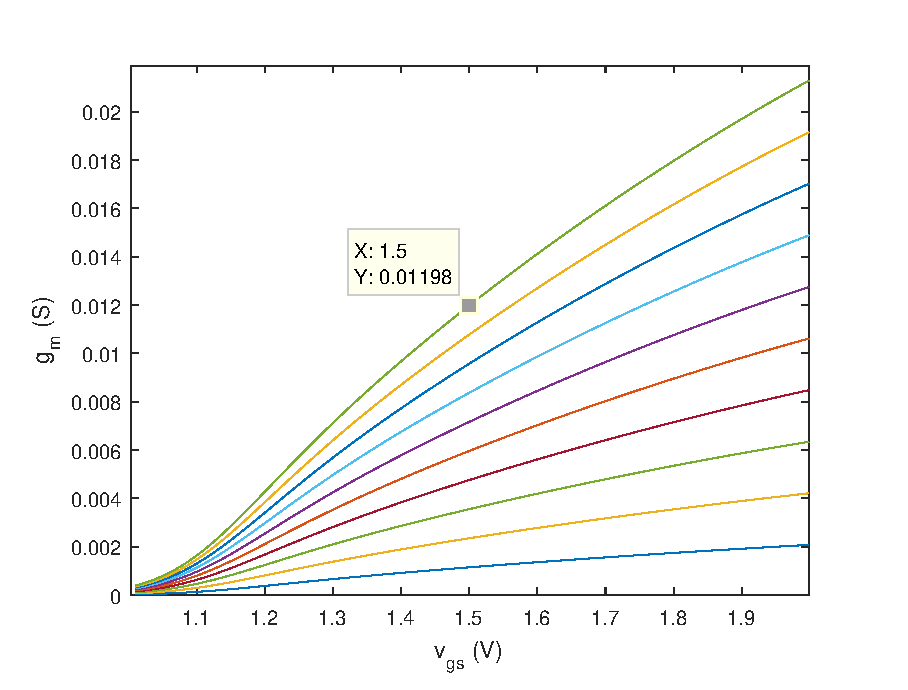
\includegraphics[scale=.6]{W2_gm}}
	\caption{ a) Drain current versus gate-source voltage of the RF stage, with W varying from 50\(\mu\)m to 500\(\mu\)m. b)Transconductance versus gate-source voltage of the RF stage, with W varying from 50\(\mu\)m to 500\(\mu\)m.}
	\label{fig:W_2_id_gm}
\end{figure}
The largest width  \(W_3=500\mu m\) (the green curve) was chosen, along with \(V_{GS3}=1.5V\), accordingly to the current and transconductance's value, eventually taking the highest values:
\begin{align}
	g_{m3}&=11.9mS \nonumber \\
	\frac{I_0}{2}&=2.9mA \nonumber
\end{align}
\begin{figure}[H]
	\centering
	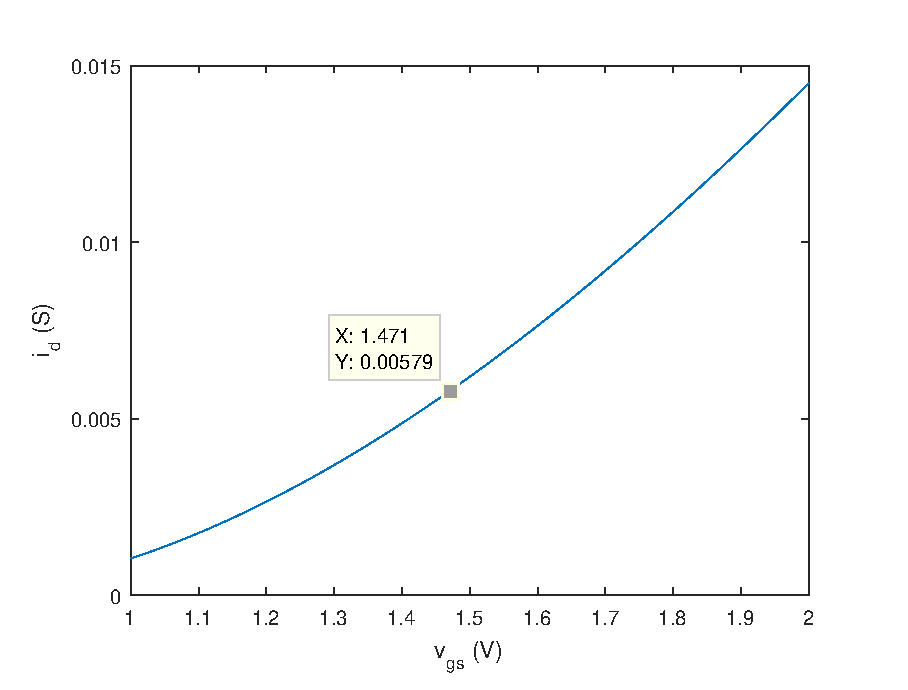
\includegraphics[scale=0.6]{W1_id}
	\caption{Drain current versus gate-source voltage of the bias transistor M1, with W=\(373\mu m\)}
	\label{W1_id}
\end{figure}
We moved then to current sink design, M1 and M2. Given the data:
\begin{align}
	V_{R_S} &= 2.9mA\cdot 10\ohm=29mV \notag \\
	V_{DS1}&=1.5V-V_{R_S}=1.471V \notag \\
	V_{GS1}&=1.471V \notag
\end{align}
This set of values leads to a width equal to \(W_1=373\mu m\) in order to have \(I_0=2\cdot2.9mA=5.8mA\) (figure \ref{W1_id}).

Finally the LO stage was designed, along with the load resistance \(R_L\) starting from the wanted conversion gain, lowered to  \(A_v=4\) with respect to what we decided in the previous section. Given the analytic expression of voltage conversion gain (Figure \ref{eq:ConvGain}):
\begin{align}
	A_v \approx \frac{2}{\pi}\left( \frac{R_L}{R_S + \frac{1}{g_{m3}}}\right)=4 \nonumber
\end{align}
The value of \(R_L\) is then determined
\begin{align}
	R_L=A_v \cdot \left( \frac{\pi}{2} \cdot\frac{1}{g_{m3}} + R_S \right)=577 \ohm
\end{align}
The drain-to-source voltage of the LO stage, \(V_{DS6}\), can be thus evaluated as follows:
\begin{align}
	V_{SB6}&=V_{DS1}+V_{R_S}+V_{DS3} \notag\\
	&= 1.47V+0.029V+1.5V=3V \nonumber
\end{align}
\begin{figure}[H]
	\centering
	\includegraphics[scale=0.6]{M6_Vth}
	\caption{Extrapolation of M6 threshold voltage from transconductance versus the \(V_{GS}\) curve. The threshold happens to be at \(1.27V\).}
	\label{M6_Vth}
\end{figure}
and 
\begin{gather}	
	V_{R_L}=2.9mA\cdot 577\ohm=1.673V \nonumber \\
	V_{DS6}=V_{dd}-V_{R_L}-V_{SB6}=327mV \nonumber
\end{gather}
The LO gate bias voltages must be slightly above the threshold, in order to let the transistors turn on and off with small LO signal variations, deviating rapidly current coming from the RF stage. To accomplish this, the transistor's threshold was extracted from simulation, using the \(g_{m}\) graph as a function of \(V_{GS}\) (figure \ref{M6_Vth}). 
Having \(V_{th6}=1.27V\), a very small overdrive of \( V_{od6}=60mV \) was chosen, for the reason reported before, and to assure the stage is not working in triode region. This leads to:
\begin{align}
	V_{GS6}=V_{th6}+V_{od6}=1.33V \nonumber
\end{align}
Once fixed the gates' voltages and the current flowing in the transistor (\(2.9mA\), due to the fact that only two transistors of LO stage conduct simultaneously), transistor width \(W_6\) was swept to fulfil precisely this biasing. The followed procedure is the same displayed in figure \ref{fig:W_2_id_gm} and the resulting dimensions are:
\begin{align}
	&W_6=170.3\mu m \nonumber\\
	&L = L_{min} = 0.6\mu m \nonumber
\end{align}                                                                      
Only for this stage the minimum channel length was taken, in order to keep small these transistors regardless overdrive small value.

                                                                                \subsection{Biasing network design}                                          From the previous section, the bias network specifications required by current sink, RF and LO stage are suddenly imposed:
\begin{align}                                                                    
	V_{G1}&=1.471 V \nonumber \\                                                    
	V_{G3}&=3 V \nonumber \\                                                        
	V_{G6}&=4.33 V \nonumber                                                        
\end{align}                                                                      
The bias network circuit employed is visible in figure \ref{fig:biasNet1}. 
\begin{figure} [H]
	\centering
	\begin{circuitikz}
		\ctikzset{tripoles/mos style/arrows,bipoles/length=1cm}
		\ctikzset{bipoles/capacitor/height=0.5}
		\ctikzset{bipoles/capacitor/width=0.1}
		%M2
		\draw (0,0) to[Tnmos,mirror,n=M2] (0,2);
		\draw (M2.source) node[left=3mm,above=3mm]{$M2$};
		\draw (M2.gate)[right] |- (M2.drain);
		\draw (M2.gate) to[short,-*] (2.5,1) node[right]{to $G_1$};
		\draw (M2.source) to[short] (0,0) node[sground]{};
		\draw (0,2) -- (-2,2) to[C=$C_{2}$] (-2,1) node[sground]{};
		%M5
		\draw (M2.drain) to[Tnmos,mirror,n=M5] (0,4.5);
		\draw (M5.source) node[left=3mm,above=3mm]{$M5$};
		\draw (M5.gate)[right] |- (M5.drain);
		\draw (0,4) -- (-2,4) to[C=$C_{1}$] (-2,3) node[sground]{};
		\draw (M5.gate) to[R, l_=$R_1$] (2,2.3) to[short,-*] (2.5,2.3) node[right]{to $G_3$};
		\draw (M5.gate) to[R=$R_1$] (2,3.7) to[short,-*] (2.5,3.7) node[right]{to $G_4$};
		%R2 R4
		\draw (M5.drain) to[R=$R_2$,n=R2] (0,6.3) to[R=$R_4$] (0,7.1) to[short,-*] (0,7.5) node[above]{$V_{dd}$};
		\draw (0,5.7) to[short] (0.7,5.7) to[R,l_=$R_3$] (2,5) to[short,-*] (2.5,5) node[right]{to $G_6$,$G_9$};
		\draw (0,5.7) to[short] (0.7,5.7) to[R=$R_3$] (2,6.4) to[short,-*] (2.5,6.4) node[right]{to $G_7$,$G_8$};
	\end{circuitikz}
	\caption{Reference biasing network schematic}
	\label{fig:biasNet1}
\end{figure}
               
The mirroring ratio for the current sink transistor M1 was chosen to be 1 as chosen in section 3. With a transistor length \(L_2 = 1.8\mu m\), and being \(V_{GS2}=V_{DS2}=1.471V\) imposed, \(W_2\) has been trimmed in the simulator to sink a current equal to \(I_0=5.8mA\), resulting in:
\begin{align}
W_2=373\mu m \notag
\end{align} 
In the same way transistor M5 width was set, in order to have a gate voltage \(V_{G5}=3V\) when stacked above M2:
\begin{align}
	W_5&=130.45\mu m \nonumber\\
	L_5&=0.6\mu m \nonumber
\end{align}
Minimum length was taken in this case to reduce the transistor's size.
The sum of \(R_2\) and \(R_4\) must be such that with total current of \(5.8mA\), the voltage drop across them is such that \(V_{G5}=3V\):
\begin{align}
	R_2+R_4=\frac{V_{dd}-V_{G5}}{I_0} = 344\ohm \nonumber
\end{align}
The partition between them must give a bias voltage to LO stage of V\textsubscript{G6}=4.33V. This brings to
\begin{align}
	R_2=229\ohm\nonumber\\
	R_4=115\ohm\nonumber
\end{align}

Resistors \(R_1\) and \(R_3\) were chosen to be large enough to isolate biasing network from RF and LO signals respectively, and form a low pass filter along with capacitors \(C_1\) and \(C_2\). Resistors were thus chosen of the order of some k\ohm.
\begin{align}
	R_1=R_3=30k\ohm \nonumber
\end{align}
From here, the minimum capacitance to filter out LO signal can be evaluated in order to have a pole at least one decade before working frequency. The output resistance of M5 has been considered negligible with respect to R\textsubscript{1} and R\textsubscript{3}, leading to an equivalent resistance for the low pass filter equal to:
\begin{align}
	R_{eq}=R_1//R_3//R_2//R4=76.4 \ohm \nonumber \\
	R_{eq} \simeq R_1||(R_2+R4||R_3)??
\end{align}
from which the resulting capacitance:
\begin{align}
	C_1\ge 10\cdot \frac{1}{2\pi \cdot R_{eq} \cdot f_{lo }} = 20.8pF
\end{align}
\(C_1 = C_2\) was chosen for simplicity. Finally a CAD optimization over them was carried on to maximize the gain and minimizing the capacitors' dimensions, leading to the final chosen value of:
\begin{align}
	C_1=C_2=25pF
\end{align}

\subsection{Validating design of the bias point}
Designed circuit has been drawn in Cadence to test it entirely. The complete test circuit is shown in figure \ref{S_cad_full}, after dc operating point simulation.
\begin{figure}[H]
	\centering
	\includegraphics[width=0.7\textwidth]{S_cad_full}
	\caption{Gilbert cell and bias network schematic}
	\label{S_cad_full}
\end{figure}

\begin{figure}[H]
	\centering
	\includegraphics[width=\textwidth]{S_cad_I0}
	\caption{Close up view on current sink and RF stage}
	\label{S_cad_I0}
\end{figure}
As it can be seen from the close-up figure \ref{S_cad_I0} bias voltages and current of the current sink M1 (N15 in Cadence schematic) are practically the same of the ones obtained in the design. Same thing can be stated for RF and LO stage in figure \ref{subfig-1:S_cad_LO} and for the biasing network (figure \ref{subfig-1:S_cad_biasnet}).
\begin{figure}[H]
	\centering
	\subfloat[Close up view of LO stage\label{subfig-1:S_cad_LO}]
	{\includegraphics[width=0.4\textwidth]{S_cad_LO}}
	\hfill
	\subfloat[Close up view of LO stage\label{subfig-1:S_cad_biasnet}]
	{\includegraphics[width=0.4\textwidth]{S_cad_biasnet}}
	\caption{}
\end{figure}

Dynamical analyses for the circuit in figure \ref{S_cad_full} have been moved in this treatise to the final chapter. In the next section circuit layout is described. \newpage
\section{Layout of the Gilbert Cell}

\newpage
\section{Simulation vs schematic comparison}

\newpage
\section{Conclusions}

The aim of this treatise was to show how to design a Gilbert cell based analog multiplier. A complete description of the GC working principle and a possible design procedure has been developed. Analysing the results obtained during the process, it is possible to notice that:
\begin{itemize}
	\item The circuit correctly performs the mixing of an input signal within bandwidth;
	\item A reasonable conversion gain has been obtained (A\textsubscript{v,layout} $\simeq$ 2.9, A\textsubscript{v,schem} $\simeq$ 2.7), having a good matching between simulations and hand calculations;
	\item The amount of distortion introduced by the net is acceptable if the input power remains well below the 1dB compression point, limiting the circuit input range to a few hundreds of millivolts though;
\end{itemize}
However, despite these encouraging outcomes we need to point out that:
\begin{itemize}
	\item The AMI's 0.6 process design kit by MOSIS is old-fashioned and not meant to be used for RF applications. Hence, the multiplier could not work correctly at the chosen frequency with the expected performances;
	\item The extractor used to generate the layout (Cadence Diva) was not able to provide the full set of parasitic elements that would appear within the circuit due to connections between components (routing, packaging) and originated by the devices themselves, leading to inaccurate analysis;
	\item A quite wide circuit area would be necessary in order to fulfil the specifications (gain, power consumption), determining the presence of large amount of parasitic elements that would worsen the circuit's performances in a real layout.  
\end{itemize}
To sum up, the circuit functions properly, although it probably overestimates what would be the real behaviour. Thus we can say, with a certain amount of confidence, that all results and circuit performances shown here, would be by far worse if implemented on a physical device.  Therefore, the design has to be intended with didactic purposes.
\\
\\
It was a great way for experimenting integrated analog design along with the use of professional cad tools. We learnt the importance of complex simulated device models in order to have functioning circuits in sub-micrometer technologies. It has been an opportunity to prove layout strategies dealing with MOSIS' integrated design rules.
\newpage


\end{document}
